% !TEX root = ../OT4ML.tex

\section{Dynamic Optimal Transport}
\label{sec-dynamic-optimal-transport}
\label{sec-wasserstein-flows}

Optimal transport becomes especially powerful once distances between measures are seen as actions of moving mass. This section first develops the dynamic language: continuity equations describe admissible measure evolutions, while the Benamou--Brenier formula identifies $\Wass_2$ with a least-action principle. These ideas prepare the gradient-flow and generative-model sections that follow.

\subsection{Evolutions over the Space of Measures}


We start with the continuity equation because it is the common language for particles, densities and weak measure evolutions. It also makes precise which velocity fields actually move mass.

\paragraph{Lagrangian and Eulerian descriptions.}

We consider the evolution $t \mapsto \alpha_t \in \Pp(\RR^d)$. Such an evolution can be described in a ``Lagrangian'' way as the advection of particles along a (time-dependent) vector field $v_t(x)$ in $\RR^d$. At the particle level, this advection is governed by
\begin{equation}
    \frac{\d x(t)}{\d t} = v_t(x(t)), \label{eq:lagrangian-advection}
\end{equation}
and we write $T_t$ for the associated flow map, so that $T_t(x(0))=x(t)$. The advected measure is then $\alpha_t = (T_t)_\sharp \alpha_0$. For discrete measures, $\alpha_t = \frac{1}{n} \sum_{i=1}^n \delta_{x_i(t)}$, meaning each $x_i(t)$ solves \eqref{eq:lagrangian-advection}.

In the Eulerian description, the same motion is written directly on the evolving measure: the particle ODE becomes the PDE
\begin{equation}
    \frac{\partial \alpha_t}{\partial t} + \diverg(v_t \alpha_t) = 0. \label{eq:eulerian-advection}
\end{equation}
This PDE is often referred to as the advection equation, the continuity equation, or Liouville's equation when operating over a phase space. For singular measures, and in particular for empirical measures, it is understood in the distributional sense:
\begin{equation}\label{eq:eulerian-advection-weak}
	\frac{\d}{\d t}\int_{\RR^d}\varphi(x)\,\d\alpha_t(x)
	=
	\int_{\RR^d}\dotp{\nabla\varphi(x)}{v_t(x)}\,\d\alpha_t(x)
\end{equation}
for every smooth compactly supported test function $\varphi$. This weak form is exactly what is obtained by differentiating $\frac1n\sum_i\varphi(x_i(t))$ when the measure is empirical.

\begin{figure}[ht]
\centering
\begin{tabular}{@{}cc@{}}
\small Lagrangian advection &
\small Eulerian flux \\[-.15em]
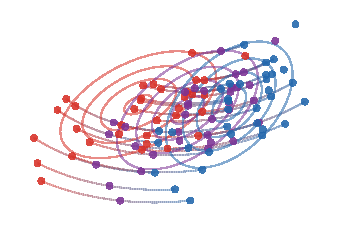
\includegraphics[width=.58\linewidth]{figures/dynamic-continuity-equation/advection.pdf} &
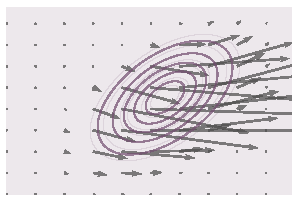
\includegraphics[width=.30\linewidth]{figures/dynamic-continuity-equation/flux.pdf}
\end{tabular}
\caption{Two views of the continuity equation. The left panel advects particles and Gaussian density contours under a smooth affine vector field, showing the Lagrangian flow $x'(t)=v(x(t))$. The right panel shows the Eulerian flux $m_t=\rho_t v_t$ at an intermediate time, where $\alpha_t=\rho_t\,\d x$: arrows are weighted by the local density, so the velocity contributes to the PDE only where mass is present.}
\label{fig:dynamic-continuity-equation}
\end{figure}

\paragraph{Benamou--Brenier action.}

The dynamic formulation of the quadratic Wasserstein distance is
\begin{equation}\label{eq:benamou-brenier}
	\Wass_2^2(\alpha_0,\alpha_1)
	=
	\inf_{\substack{\partial_t\alpha_t+\diverg(\alpha_t v_t)=0\\
	\alpha_{t=0}=\alpha_0,\ \alpha_{t=1}=\alpha_1}}
	\int_0^1\!\int_{\RR^d}\norm{v_t(x)}^2\,\d\alpha_t(x)\,\d t.
\end{equation}
For a prescribed smooth curve $(\alpha_t)_t$, the tangent velocity of minimal kinetic energy is the solution of the constrained least-squares problem
\begin{equation}\label{eq:least-square-field}
	v_t
	=
	\argmin_{v}
	\enscond{\int\norm{v(x)}^2\,\d\alpha_t(x)}
	{\partial_t\alpha_t+\diverg(\alpha_t v)=0}.
\end{equation}
If $\alpha_t=\rho_t\,\d x$ is a smooth positive density, this minimizer is a gradient field $v_t=\nabla\varphi_t$ where
\begin{equation}\label{eq:least-square-field-explicit}
	-\diverg(\rho_t\nabla\varphi_t)=\partial_t\rho_t.
\end{equation}


While this is not the focus of this chapter, let us note that although the formulation~\eqref{eq:benamou-brenier} is not jointly convex in $(\alpha_t,v_t)$, for density curves $\alpha_t=\rho_t\,\d x$ the change of variable $m_t:=\rho_t v_t$ gives the convex perspective form
\[
	\Wass_2^2(\alpha_0,\alpha_1)
	=
	\inf_{\substack{\partial_t\rho_t+\diverg m_t=0\\
	\rho_{t=0}\d x=\alpha_0,\ \rho_{t=1}\d x=\alpha_1}}
	\int_0^1\!\int_{\RR^d}
	\frac{\norm{m_t(x)}^2}{\rho_t(x)}\,\d x\,\d t,
\]
with the usual convention that the integrand is $0$ when $(\rho_t,m_t)=(0,0)$ and $+\infty$ when $\rho_t=0$ but $m_t\neq0$. This convex reformulation enables geodesic interpolation by convex optimization once the domain is discretized.

\begin{figure}[ht]
\centering
\begin{tabular}{@{}cc@{}}
\small density sequence &
\small midpoint velocities \\[-.15em]

\includegraphics[width=.58\linewidth]{figures/dynamic-benamou-brenier-geodesic/density-sequence.pdf} &

\includegraphics[width=.30\linewidth]{figures/dynamic-benamou-brenier-geodesic/midpoint-velocities.pdf}
\end{tabular}
\caption{Benamou--Brenier geodesic between two sampled silhouettes. A discrete quadratic OT plan between the cat and two-disks point clouds induces the McCann interpolation $Z_t=(1-t)X+tY$, which is the Lagrangian realization of the least-action solution. The left panel shows kernel-density contours along this geodesic, and the right panel displays midpoint particles with their constant characteristic velocities $Y-X$.}
\label{fig:dynamic-benamou-brenier-geodesic}
\end{figure}

\begin{rem}[Path-space formulation]
Let $\Ss=C([0,1];\RR^d)$ be the space of continuous paths endowed with the uniform topology. For $t\in[0,1]$ define the evaluation map
\[
P_t: \Ss\to\RR^d,\qquad P_t(\gamma)=\gamma(t).
\]
The Benamou--Brenier cost admits the equivalent formulation over probability measures concentrated on absolutely continuous paths,
\[
\Wass_2^2(\alpha_0,\alpha_1)=\inf_{M\in\Pp(\Ss)}\Bigl\{\int_{\Ss}\!\int_0^1|\dot\gamma(t)|^2\,\d t\,\d M(\gamma): (P_0)_{\sharp}M=\alpha_0,\ (P_1)_{\sharp}M=\alpha_1\Bigr\}.
\]
If $\alpha_0$ has a density, the minimizer $M^*$ is unique. Its time marginals reproduce the optimal curve: $\alpha_t=(P_t)_{\sharp}M^*$ for all $t$. Furthermore, for a.e. $t$, denoting $Q_t(\gamma)=\dot\gamma(t)$ on the absolutely continuous paths where this derivative is defined, the conditional law of the velocity is deterministic:
\[
(P_t,Q_t)_\sharp M^*(\d x,\d q)=\alpha_t(\d x)\delta_{v_t^*(x)}(\d q),
\]
where $v_t^*$ is the optimal velocity field in the Benamou--Brenier formulation. Hence $M^*$ concentrates on straight-line geodesics and, for a.e. $t$, assigns exactly one direction at $\alpha_t$-a.e. spatial point.
\end{rem}

\subsection{Extensions of the Dynamic Formulation}
\label{sec-bb-extensions}

The same variational grammar extends beyond the quadratic Wasserstein distance. One changes either the kinetic exponent, the mobility or the balance equation, while keeping a continuity-type constraint and a convex perspective action.

\begin{rem}[Generalized Benamou--Brenier distances]\label{rem-generalized-bb}
	The dynamic formulation is not specific to $\Wass_2$. For measures with finite $p$-th moments and $p>1$, one has the analogous action formula
	\[
		\Wass_p^p(\alpha_0,\alpha_1)
		=
		\inf_{\substack{\partial_t\alpha_t+\nabla\!\cdot(\alpha_t v_t)=0\\
		\alpha_{t=0}=\alpha_0,\ \alpha_{t=1}=\alpha_1}}
		\int_0^1\!\int_{\RR^d} |v_t(x)|^p\,\d\alpha_t(x)\,\d t.
	\]
	When $\alpha_t=\rho_t\,\d x$ and $m_t=\rho_t v_t$, this becomes the convex perspective action
	\[
		\int_0^1\!\int_{\RR^d}
		\frac{|m_t(x)|^p}{\rho_t(x)^{p-1}}\,\d x\,\d t,
		\qquad
		\partial_t\rho_t+\nabla\!\cdot m_t=0,
	\]
	with the usual convention that the integrand is $0$ if $(\rho,m)=(0,0)$ and $+\infty$ if $\rho=0$ but $m\neq0$.

	A second class of variants changes the mobility of the medium: the quadratic action $|m|^2/\rho$ is replaced by $|m|^2/\theta(\rho)$ for a suitable concave mobility $\theta$. Under appropriate structural assumptions, this produces transport metrics adapted to nonlinear diffusions and finite-volume discretizations~\cite{dolbeault2009new}. On finite graphs and Markov chains, the analogous action uses an edge mobility, often the logarithmic mean of the endpoint densities, and leads to discrete Wasserstein geometries~\cite{Maas2011,MielkeCVPDE}. A third class allows creation and destruction of mass by replacing the continuity equation by a balance equation and penalizing both transport and growth. A representative quadratic action is
	\[
		\partial_t\rho_t+\nabla\!\cdot m_t=s_t,
		\qquad
		\int_0^1\!\int
		\left(\frac{|m_t|^2}{\rho_t}+\kappa^2\frac{s_t^2}{\rho_t}\right)\d x\,\d t,
	\]
	with the same perspective convention. This leads, up to normalization conventions, to the Wasserstein--Fisher--Rao or Hellinger--Kantorovich geometry for unbalanced measures~\cite{LieroMielkeSavareLong,2015-chizat-unbalanced,2017-chizat-focm}. These extensions keep the same variational grammar as Benamou--Brenier: a balance equation, an action density, and geodesics obtained by minimizing an integrated kinetic cost.
\end{rem}
